\begin{frame}{目录}
    \tableofcontents
\end{frame}

\section{贝尔曼公式}

\begin{frame}{标注说明}
    考虑以下单步过程:
    \[
        S_t\xrightarrow{A_t}R_{t+1},S_{t+1}
    \]
    \begin{itemize}
        \item $t,t+1$:离散时间序列
        \item $S_t$:在时刻$t$的状态
        \item $A_t$:在时刻$t$的动作
        \item $R_{t+1}$:执行完$A_t$之后的奖励
        \item $S_{t+1}$:执行完$A_t$之后的状态
    \end{itemize}
    注意$S_t,A_t,R_{t+1}$都是随机变量。

    \begin{itemize}
        \item $A_t\sim \pi(A_t|S_t=s)$
        \item $R_{t+1}\sim p(R_{t+1}|S_t=s,A_t=a)$
        \item $S_{t+1}\sim p(S_{t+1}|S_t=s,A_t=a)$
    \end{itemize}
    假设所有的上述概率分布(系统模型)都是已知的。
\end{frame}

\begin{frame}{标注说明}
    考虑以下轨迹:
    \[
        S_t\xrightarrow{A_t}R_{t+1},S_{t+1}\xrightarrow{A_{t+1}}R_{t+2},S_{t+2}\xrightarrow{A_{t+2}}R_{t+3},\cdots
    \]
    其折扣回报为:
    \[
        G_t=R_{t+1}+\gamma R_{t+2}+\gamma^2 R_{t+3}+\cdots
    \]
    \begin{itemize}
        \item $\gamma\in(0,1)$:折扣系数
        \item $G_t$:也是一个随机变量,因为$R_{t+1},R_{t+2},\cdots$都是随机变量
    \end{itemize}
\end{frame}

\begin{frame}{状态价值}
    $G_t$的数学期望值被称为\textbf{状态价值}。
    \[
        v_{\pi}(s)=\mathbbm{E}[G_t|S_t=s]
    \]
    \begin{itemize}
        \item 它是一个$s$的函数。它是当状态处于$s$时的条件期望。
        \item 它是一个$\pi$的函数。对于不同的策略,状态价值是不同的。
    \end{itemize}
    问题:状态价值和回报的关系是什么?

    答:状态价值是从一个状态出发得到的回报的期望值。
\end{frame}

\begin{frame}{状态价值}
    从$s_1$出发下面哪一个策略最好?
    \begin{center}
        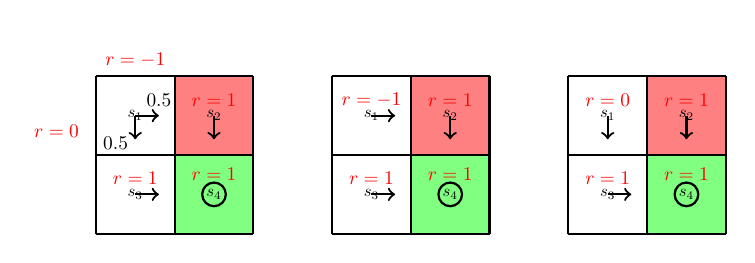
\begin{tikzpicture}
            % 填充指定格子为红色
            \fill[red!50] (1,1) rectangle (2,2); % 第2行第3列 (索引 (2,1))
            \fill[green!50] (1,0) rectangle (2,1); % 第3行第1列 (索引 (0,0))

            % 画3x3网格
            \draw[thick] (0,0) grid (2,2);
            
            % 标记状态编号 (行列索引)
            \foreach \x in {0,1,2} {
                \foreach \y in {0,1,2} {
                    \node at (\x+0.5, 2.5-\y){};
                }
            }
            
            % 绘制箭头表示策略
            % 示例:在格子中绘制箭头

           % 从 s_4 (0, 1) 向下
           \draw[->, thick] (0.5, 1.5) -- (0.8, 1.5); % 向下

           % 从 s_5 (1, 1) 向右
           \draw[->, thick] (1.5, 1.5) -- (1.5, 1.2); % 向右


           % 从 s_7 (0, 2) 向右
           \draw[->, thick] (0.5, 0.5) -- (0.8, 0.5); % 向右

           % 从 s_9 (2, 2) 向左
           \draw[thick] (1.5, 0.5) circle (0.15);
            \node[scale=0.6] at (0.5, 1.5) {$s_1$};
            \node[scale=0.6] at (1.5, 1.5) {$s_2$};
            \node[scale=0.6] at (0.5, 0.5) {$s_3$};
            \node[scale=0.6] at (1.5, 0.5) {$s_4$};

            \node[scale=0.7, color=red] at (0.5, 1.7) {$r=-1$};
            \node[scale=0.7, color=red] at (1.5, 1.7) {$r=1$};
            \node[scale=0.7, color=red] at (0.5, 0.7) {$r=1$};
            \node[scale=0.7, color=red] at (1.5, 0.75) {$r=1$};
            % 填充指定格子为红色
            \fill[red!50] (-2,1) rectangle (-1,2); % 第2行第3列 (索引 (2,1))
            \fill[green!50] (-2,0) rectangle (-1,1); % 第3行第1列 (索引 (0,0))

            % 画3x3网格
            \draw[thick] (-3,0) grid (-1,2);
            
            % 标记状态编号 (行列索引)
            \foreach \x in {0,1,2} {
                \foreach \y in {0,1,2} {
                    \node at (\x+0.5, 2.5-\y){};
                }
            }
            
            % 绘制箭头表示策略
            % 示例:在格子中绘制箭头

            % 从 s_1 (0, 0) 向右的箭头
            \draw[->, thick] (-2.5, 1.5) -- (-2.2, 1.5); % 向右
            \node[scale=0.7] at (-2.2, 1.7) {0.5}; % 在箭头上方标注 50%
            \draw[->, thick] (-2.5, 1.5) -- (-2.5, 1.2);
            \node[scale=0.7] at (-2.75, 1.15) {0.5}; % 在箭头右侧标注 50%

           % 从 s_5 (1, 1) 向右
           \draw[->, thick] (-1.5, 1.5) -- (-1.5, 1.2); % 向右


           % 从 s_7 (0, 2) 向右
           \draw[->, thick] (-2.5, 0.5) -- (-2.2, 0.5); % 向右

           % 从 s_9 (2, 2) 向左
           \draw[thick] (-1.5, 0.5) circle (0.15);
            \node[scale=0.6] at (-2.5, 1.5) {$s_1$};
            \node[scale=0.6] at (-1.5, 1.5) {$s_2$};
            \node[scale=0.6] at (-2.5, 0.5) {$s_3$};
            \node[scale=0.6] at (-1.5, 0.5) {$s_4$};

            \node[scale=0.7, color=red] at (-2.5, 2.2) {$r=-1$};
            \node[scale=0.7, color=red] at (-3.5, 1.3) {$r=0$};
            \node[scale=0.7, color=red] at (-1.5, 1.7) {$r=1$};
            \node[scale=0.7, color=red] at (-2.5, 0.7) {$r=1$};
            \node[scale=0.7, color=red] at (-1.5, 0.75) {$r=1$};
            % 填充指定格子为红色
            \fill[red!50] (4,1) rectangle (5,2); % 第2行第3列 (索引 (2,1))
            \fill[green!50] (4,0) rectangle (5,1); % 第3行第1列 (索引 (0,0))

            % 画3x3网格
            \draw[thick] (3,0) grid (5,2);
            
            % 标记状态编号 (行列索引)
            \foreach \x in {0,1,2} {
                \foreach \y in {0,1,2} {
                    \node at (\x+0.5, 2.5-\y){};
                }
            }
            
            % 绘制箭头表示策略
            % 示例:在格子中绘制箭头

           % 从 s_4 (0, 1) 向下
           \draw[->, thick] (3.5, 1.5) -- (3.5, 1.2); % 向下

           % 从 s_5 (1, 1) 向右
           \draw[->, thick] (4.5, 1.5) -- (4.5, 1.2); % 向右


           % 从 s_7 (0, 2) 向右
           \draw[->, thick] (3.5, 0.5) -- (3.8, 0.5); % 向右

           % 从 s_9 (2, 2) 向左
           \draw[thick] (4.5, 0.5) circle (0.15);
            \node[scale=0.6] at (3.5, 1.5) {$s_1$};
            \node[scale=0.6] at (4.5, 1.5) {$s_2$};
            \node[scale=0.6] at (3.5, 0.5) {$s_3$};
            \node[scale=0.6] at (4.5, 0.5) {$s_4$};

            \node[scale=0.7, color=red] at (3.5, 1.7) {$r=0$};
            \node[scale=0.7, color=red] at (4.5, 1.7) {$r=1$};
            \node[scale=0.7, color=red] at (3.5, 0.7) {$r=1$};
            \node[scale=0.7, color=red] at (4.5, 0.75) {$r=1$};
        \end{tikzpicture}
    \end{center}
    \[
        \begin{aligned}
            v_{\pi_1}(s_1)&=0.5\left(-1+\frac{\gamma}{1-\gamma}\right)+0.5\left(\frac{\gamma}{1-\gamma}\right) = -0.5+\frac{\gamma}{1-\gamma}\\
            v_{\pi_2}(s_1)&=-1+\gamma1+\gamma^21+\cdots=-1+\frac{\gamma}{1-\gamma}\\
            v_{\pi_3}(s_1)&=0+\gamma1+\gamma^21+\cdots=\frac{\gamma}{1-\gamma} \\            
        \end{aligned}
    \]
\end{frame}

\begin{frame}{贝尔曼公式}
    如何计算状态价值$v_{\pi}(s)$?
    \[
        \begin{aligned}
            \alert{v_\pi(s)}&=\mathbbm{E}[R_{t+1}|S_t=s]+\gamma\mathbbm{E}[G_{t+1}|S_t=s] \\
            &=\sum_a\pi(a|s)\sum_r p(r|s,a)r+\gamma\sum_a\pi(a|s)\sum_{s'}p(s'|s,a)\alert{v_{\pi}(s')} \\
            &=\sum_a\pi(a|s)\left[\sum_r p(r|s,a)r+\gamma\sum_{s'}p(s'|s,a)\alert{v_{\pi}(s')}\right], \quad \forall s\in\mathcal{S}
        \end{aligned}
    \]
    \begin{itemize}
        \item 以上方程被称作贝尔曼公式。它描述了不同状态价值之间的关系。
        \item 它由两项组成:一项是即时奖励,一项是长期奖励。
        \item 贝尔曼公式实际上是一组方程,每一个状态都有它对应的贝尔曼公式。
    \end{itemize}
\end{frame}

\begin{frame}{贝尔曼公式}
    考虑以下策略:
    \begin{center}
        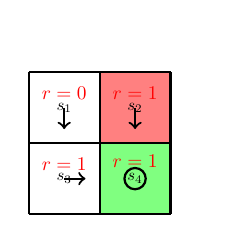
\begin{tikzpicture}[scale=0.9]
            % 填充指定格子为红色
            \fill[red!50] (1,1) rectangle (2,2); % 第2行第3列 (索引 (2,1))
            \fill[green!50] (1,0) rectangle (2,1); % 第3行第1列 (索引 (0,0))

            % 画3x3网格
            \draw[thick] (0,0) grid (2,2);
            
            % 标记状态编号 (行列索引)
            \foreach \x in {0,1,2} {
                \foreach \y in {0,1,2} {
                    \node at (\x+0.5, 2.5-\y){};
                }
            }
            
            % 绘制箭头表示策略
            % 示例:在格子中绘制箭头

           % 从 s_4 (0, 1) 向下
           \draw[->, thick] (0.5, 1.5) -- (0.5, 1.2); % 向下

           % 从 s_5 (1, 1) 向右
           \draw[->, thick] (1.5, 1.5) -- (1.5, 1.2); % 向右


           % 从 s_7 (0, 2) 向右
           \draw[->, thick] (0.5, 0.5) -- (0.8, 0.5); % 向右

           % 从 s_9 (2, 2) 向左
           \draw[thick] (1.5, 0.5) circle (0.15);
            \node[scale=0.6] at (0.5, 1.5) {$s_1$};
            \node[scale=0.6] at (1.5, 1.5) {$s_2$};
            \node[scale=0.6] at (0.5, 0.5) {$s_3$};
            \node[scale=0.6] at (1.5, 0.5) {$s_4$};

            \node[scale=0.7, color=red] at (0.5, 1.7) {$r=0$};
            \node[scale=0.7, color=red] at (1.5, 1.7) {$r=1$};
            \node[scale=0.7, color=red] at (0.5, 0.7) {$r=1$};
            \node[scale=0.7, color=red] at (1.5, 0.75) {$r=1$};
        \end{tikzpicture}
    \end{center}
    贝尔曼公式:
    \[
        \alert{v_\pi(s)}=\sum_a\pi(a|s)\left[\sum_r p(r|s,a)r+\gamma\sum_{s'}p(s'|s,a)\alert{v_{\pi}(s')}\right], \quad \forall s\in\mathcal{S}
    \]
    $s_1$的状态价值:
    \begin{itemize}
        \item $\pi(a=a_3|s_1)=1$且$\pi(a\neq a_3|s_1)=0$
        \item $p(s'=s_3|s_1,a_3)=1$且$p(s'|s_1,a\neq a_3)=0$
        \item $p(r=0|s_1,a_3)=1$且$p(r\neq 0|s_1, a_3)=0$
        \item $v_\pi(s_1)=0+\gamma v_\pi(s_3)$
    \end{itemize}

\end{frame}

\begin{frame}{贝尔曼公式}
    贝尔曼公式:
    \[
        \alert{v_\pi(s)}=\sum_a\pi(a|s)\left[\sum_r p(r|s,a)r+\gamma\sum_{s'}p(s'|s,a)\alert{v_{\pi}(s')}\right], \quad \forall s\in\mathcal{S}
    \]
    同理可得(取$\gamma=0.9$):
    \[
        \begin{aligned}
            v_\pi(s_1)&=0+\gamma v_\pi(s_3)=\frac{\gamma}{1-\gamma}=9 \\
            v_\pi(s_2)&=1+\gamma v_\pi(s_4)=\frac{1}{1-\gamma}=10 \\
            v_\pi(s_3)&=1+\gamma v_\pi(s_3)=\frac{1}{1-\gamma}=10 \\
            v_\pi(s_4)&=1+\gamma v_\pi(s_4)=\frac{1}{1-\gamma}=10\\
        \end{aligned}
    \]

\end{frame}

\begin{frame}{贝尔曼公式的矩阵-向量形式}
    每次计算状态价值都要为每个状态列一个方程求解,比较麻烦。可以采用贝尔曼公式的矩阵-向量形式简化。
    可以先将贝尔曼公式:
    \[
        v_\pi(s)=\sum_a\pi(a|s)\left[\sum_r p(r|s,a)r+\gamma\sum_{s'}p(s'|s,a)v_{\pi}(s')\right]
    \]
    写为:
    \[
        v_\pi(s)=r_\pi(s)+\gamma\sum_{s'}p_\pi(s'|s)v_\pi(s')
    \]
    其中:
    \[
        r_\pi(s)=\sum_a\pi(a|s)\sum_r p(r|s,a)r, \quad p_\pi(s'|s)=\sum_a\pi(a|s)p(s'|s,a)
    \]
    然后就可以得到矩阵-向量形式:
    \[
        v_\pi=r_\pi+\gamma P_\pi v_\pi
    \]
\end{frame} 

\begin{frame}{贝尔曼公式的矩阵-向量形式}
    假设一共有4个状态,$v_\pi=r_\pi+\gamma P_\pi v_\pi$可以被写作:
    \[
       \begin{bmatrix}
            v_\pi(s_1) \\
            v_\pi(s_2) \\
            v_\pi(s_3) \\
            v_\pi(s_4) \\
        \end{bmatrix}
        =
        \begin{bmatrix}
            r_\pi(s_1) \\
            r_\pi(s_2) \\
            r_\pi(s_3) \\
            r_\pi(s_4) \\
        \end{bmatrix}
        +
        \gamma
        \begin{bmatrix}
            p_\pi(s_1|s_1) & p_\pi(s_2|s_1) & p_\pi(s_3|s_1) & p_\pi(s_4|s_1) \\
            p_\pi(s_1|s_2) & p_\pi(s_2|s_2) & p_\pi(s_3|s_2) & p_\pi(s_4|s_2) \\
            p_\pi(s_1|s_3) & p_\pi(s_2|s_3) & p_\pi(s_3|s_3) & p_\pi(s_4|s_3) \\
            p_\pi(s_1|s_4) & p_\pi(s_2|s_4) & p_\pi(s_3|s_4) & p_\pi(s_4|s_4) \\
        \end{bmatrix}
        \begin{bmatrix}
            v_\pi(s_1) \\
            v_\pi(s_2) \\
            v_\pi(s_3) \\
            v_\pi(s_4) \\
        \end{bmatrix}
    \]
    \begin{center}
        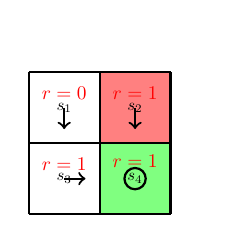
\begin{tikzpicture}[scale=0.9]
            % 填充指定格子为红色
            \fill[red!50] (1,1) rectangle (2,2); % 第2行第3列 (索引 (2,1))
            \fill[green!50] (1,0) rectangle (2,1); % 第3行第1列 (索引 (0,0))

            % 画3x3网格
            \draw[thick] (0,0) grid (2,2);
            
            % 标记状态编号 (行列索引)
            \foreach \x in {0,1,2} {
                \foreach \y in {0,1,2} {
                    \node at (\x+0.5, 2.5-\y){};
                }
            }
            
            % 绘制箭头表示策略
            % 示例:在格子中绘制箭头

           % 从 s_4 (0, 1) 向下
           \draw[->, thick] (0.5, 1.5) -- (0.5, 1.2); % 向下

           % 从 s_5 (1, 1) 向右
           \draw[->, thick] (1.5, 1.5) -- (1.5, 1.2); % 向右


           % 从 s_7 (0, 2) 向右
           \draw[->, thick] (0.5, 0.5) -- (0.8, 0.5); % 向右

           % 从 s_9 (2, 2) 向左
           \draw[thick] (1.5, 0.5) circle (0.15);
            \node[scale=0.6] at (0.5, 1.5) {$s_1$};
            \node[scale=0.6] at (1.5, 1.5) {$s_2$};
            \node[scale=0.6] at (0.5, 0.5) {$s_3$};
            \node[scale=0.6] at (1.5, 0.5) {$s_4$};

            \node[scale=0.7, color=red] at (0.5, 1.7) {$r=0$};
            \node[scale=0.7, color=red] at (1.5, 1.7) {$r=1$};
            \node[scale=0.7, color=red] at (0.5, 0.7) {$r=1$};
            \node[scale=0.7, color=red] at (1.5, 0.75) {$r=1$};
        \end{tikzpicture}
    \end{center}
    \[
       \begin{bmatrix}
            v_\pi(s_1) \\
            v_\pi(s_2) \\
            v_\pi(s_3) \\
            v_\pi(s_4) \\
        \end{bmatrix}
        =
        \begin{bmatrix}
            0 \\
            1 \\
            1 \\
            1 \\
        \end{bmatrix}
        +
        \gamma
        \begin{bmatrix}
            0 & 0 & 1 & 0 \\
            0 & 0 & 0 & 1 \\
            0 & 0 & 0 & 1 \\
            0 & 0 & 0 & 1 \\
        \end{bmatrix}
        \begin{bmatrix}
            v_\pi(s_1) \\
            v_\pi(s_2) \\
            v_\pi(s_3) \\
            v_\pi(s_4) \\
        \end{bmatrix}
    \]

\end{frame} 

\begin{frame}{动作价值}
    从状态价值到动作价值:
    \begin{itemize}
        \item 状态价值:智能体从一个状态出发得到的回报的期望值
        \item \textbf{动作价值}:智能体从一个状态出发执行了一个动作之后得到的回报的期望值
    \end{itemize}
    动作价值可以让我们知道在一个状态下采取哪个动作更好。
\end{frame}

\begin{frame}{动作价值}
    定义:
    \[
        q_\pi(s,a)=\mathbbm{E}[G_t|S_t=s,A_t=a]
    \]
    \begin{itemize}
        \item $q$是一个“状态-动作”对的函数。
        \item $q$是一个$\pi$的函数。对于不同的策略,动作价值是不同的。
    \end{itemize}
    它服从条件期望的公式:
    \begin{equation}
        \mathbbm{E}[G_t|S_t=s]=\sum_a\mathbbm{E}[G_t|S_t=s,A_t=a]\pi(a|s)
    \end{equation}
    所以:
    \begin{equation}
        \alert{v_\pi(s)}=\sum_a \pi(a|s)\alert{q_\pi(s,a)}
    \end{equation}
\end{frame}

\begin{frame}{动作价值}
    贝尔曼公式:
    \begin{equation}
        \alert{v_\pi(s)}=\sum_a\pi(a|s)\left[\sum_r p(r|s,a)r+\gamma\sum_{s'}p(s'|s,a)\alert{v_{\pi}(s')}\right]
    \end{equation}
    所以可以发现:
    \begin{equation}
        \alert{q_\pi(s,a)}=\sum_r p(r|s,a)r+\gamma\sum_{s'}p(s'|s,a)\alert{v_{\pi}(s')}
    \end{equation}
    \begin{itemize}
        \item (2)式表达了如何用动作价值计算状态价值
        \item (4)式表达了如何用状态价值计算动作价值
    \end{itemize}
\end{frame}

\begin{frame}{动作价值}
    \begin{center}
        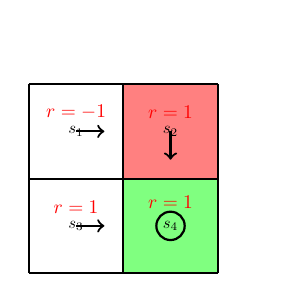
\begin{tikzpicture}[scale=1.2]
            % 填充指定格子为红色
            \fill[red!50] (1,1) rectangle (2,2); % 第2行第3列 (索引 (2,1))
            \fill[green!50] (1,0) rectangle (2,1); % 第3行第1列 (索引 (0,0))

            % 画3x3网格
            \draw[thick] (0,0) grid (2,2);
            
            % 标记状态编号 (行列索引)
            \foreach \x in {0,1,2} {
                \foreach \y in {0,1,2} {
                    \node at (\x+0.5, 2.5-\y){};
                }
            }
            
            % 绘制箭头表示策略
            % 示例:在格子中绘制箭头

           % 从 s_4 (0, 1) 向下
           \draw[->, thick] (0.5, 1.5) -- (0.8, 1.5); % 向下

           % 从 s_5 (1, 1) 向右
           \draw[->, thick] (1.5, 1.5) -- (1.5, 1.2); % 向右


           % 从 s_7 (0, 2) 向右
           \draw[->, thick] (0.5, 0.5) -- (0.8, 0.5); % 向右

           % 从 s_9 (2, 2) 向左
           \draw[thick] (1.5, 0.5) circle (0.15);
            \node[scale=0.6] at (0.5, 1.5) {$s_1$};
            \node[scale=0.6] at (1.5, 1.5) {$s_2$};
            \node[scale=0.6] at (0.5, 0.5) {$s_3$};
            \node[scale=0.6] at (1.5, 0.5) {$s_4$};

            \node[scale=0.7, color=red] at (0.5, 1.7) {$r=-1$};
            \node[scale=0.7, color=red] at (1.5, 1.7) {$r=1$};
            \node[scale=0.7, color=red] at (0.5, 0.7) {$r=1$};
            \node[scale=0.7, color=red] at (1.5, 0.75) {$r=1$};
        \end{tikzpicture}
    \end{center}
    写出$s_1$的动作价值:
    \[
        q_\pi(s_1,a_2)=-1+\gamma v_\pi(s_2)
    \]
    问题:
    \begin{itemize}
        \item $q_\pi(s_1,a_1),q_\pi(s_1,a_3),q_\pi(s_1,a_4),q_\pi(s_1,a_5)$分别是多少?
    \end{itemize}
\end{frame}

\begin{frame}{动作价值}
    \begin{center}
        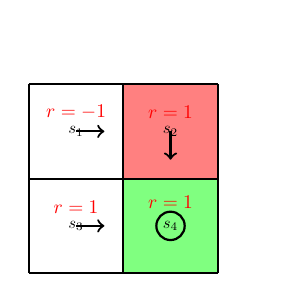
\begin{tikzpicture}[scale=1.2]
            % 填充指定格子为红色
            \fill[red!50] (1,1) rectangle (2,2); % 第2行第3列 (索引 (2,1))
            \fill[green!50] (1,0) rectangle (2,1); % 第3行第1列 (索引 (0,0))

            % 画3x3网格
            \draw[thick] (0,0) grid (2,2);
            
            % 标记状态编号 (行列索引)
            \foreach \x in {0,1,2} {
                \foreach \y in {0,1,2} {
                    \node at (\x+0.5, 2.5-\y){};
                }
            }
            
            % 绘制箭头表示策略
            % 示例:在格子中绘制箭头

           % 从 s_4 (0, 1) 向下
           \draw[->, thick] (0.5, 1.5) -- (0.8, 1.5); % 向下

           % 从 s_5 (1, 1) 向右
           \draw[->, thick] (1.5, 1.5) -- (1.5, 1.2); % 向右


           % 从 s_7 (0, 2) 向右
           \draw[->, thick] (0.5, 0.5) -- (0.8, 0.5); % 向右

           % 从 s_9 (2, 2) 向左
           \draw[thick] (1.5, 0.5) circle (0.15);
            \node[scale=0.6] at (0.5, 1.5) {$s_1$};
            \node[scale=0.6] at (1.5, 1.5) {$s_2$};
            \node[scale=0.6] at (0.5, 0.5) {$s_3$};
            \node[scale=0.6] at (1.5, 0.5) {$s_4$};

            \node[scale=0.7, color=red] at (0.5, 1.7) {$r=-1$};
            \node[scale=0.7, color=red] at (1.5, 1.7) {$r=1$};
            \node[scale=0.7, color=red] at (0.5, 0.7) {$r=1$};
            \node[scale=0.7, color=red] at (1.5, 0.75) {$r=1$};
        \end{tikzpicture}
    \end{center}
    \begin{itemize}
        \item 动作价值比较关键的原因是我们最关心的其实是要做什么动作。
        \item 我们可以先把所有状态价值都算出来,然后再算所有的动作价值
        \item \alert{即使没有模型,我们也可以估计动作价值}。
    \end{itemize}
\end{frame}

\begin{frame}{小结}
    关键概念和结论:
    \begin{itemize}
        \item 状态价值:$v_\pi(s)=\mathbbm{E}[G_t|S_t=s]$
        \item 动作价值:$q_\pi(s,a)=\mathbbm{E}[G_t|S_t=s,A_t=a]$
        \item 贝尔曼公式:
        \[
            \begin{aligned}
                \alert{v_\pi(s)}&=\sum_a\pi(a|s)\left[\sum_r p(r|s,a)r+\gamma\sum_{s'}p(s'|s,a)\alert{v_{\pi}(s')}\right] \\
                &=\sum_a\pi(a|s)\alert{q_\pi(s,a)}
            \end{aligned}
        \]
    \end{itemize}
\end{frame}
